\documentclass{../source/Experiment}

\major{信息工程}
\name{姚桂涛}
\title{波导传输线负载特性测量与阻抗匹配}
\stuid{3190105597}
\college{信息与电子工程学院}
\date{\today}
\lab{东4-221}
\course{电磁场与电磁波}
\instructor{王子立}
\grades{}
\expname{波导传输线负载特性测量与阻抗匹配}
\exptype{}
\partner{华天择}

\usepackage{caption}

\DeclareCaptionLabelSeparator{twospace}{\, }
\captionsetup{labelsep = twospace}

\begin{document}
    \makecover
    \makeheader

    \section{实验目的}
    了解波导传输线的基本特性,容性膜片的负载特性及阻抗匹配方法。
    
    覆盖的基本概念:
    \begin{itemize}
        \item 波导的传输线模型
        \item 波导色散特性——波导波长
        \item 阻抗及匹配
        \item Smith圆图
    \end{itemize}

    \section{实验过程及结果}

        \subsection{工作频率ƒ测量}
            \begin{enumerate}
                \item 测量线开口端用短路块短接。
                \item 接通固态微波信号源,工作状态选择方波调制。
                \item 调节波导检波器中的短路活塞或三销钉调配器使示波器上显示的检波输出(方波)幅度最大。如果示波器上显示的输出幅度还不够大,可适当减少可调衰减器的衰减量,反之增加可调衰减器的衰减量。(注意:由于微波频率高,波长短,故调节时必须如同调节显微镜一样细心,而且在用三销钉调节时,销钉插入深度不能超过波导高度b 的一半,否则会产生全反射以至无信号检出。)
                \item 用直读式频率计测量此时系统的工作频率ƒ(注意:调节时必须缓慢细调,由于频率计等效于电路中的一个并联谐振回路,当它产生谐振时,一部份能量被吸收,相应地串接在后面的检波器得到的能量就变小,于是示波器上看 到的方波幅度也就变小,因而调节时注意观察示波器上的方波幅度, 当看到幅度有突变,且变得最小时,频率计上读得的读数就是微波信号源的振荡频率,单位为GHz。频率计的读法是:两条水平红线夹着的那一行刻度线与垂直红线相交的那一点的刻度数值),记录到实验记录本上。
            \end{enumerate}

            \begin{figure}[H]
                \centering
                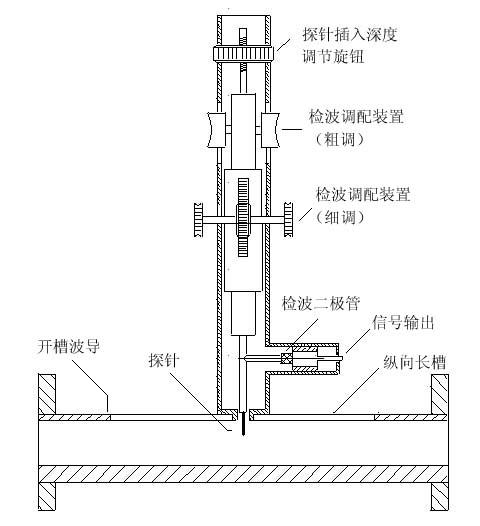
\includegraphics[width = 0.4\textwidth]{pic/波导驻波测量线结构示意}
                \caption{波导驻波测量线结构示意}
            \end{figure}

        \subsection{波导波长测量}
            \begin{enumerate}
                \item 先调节测量线探针插入深度为1mm 左右,再细心调节测量线上的检波调配装置,使数字万用表上指示的检波输出信号最大,即检波匹配(注意:为使测量线的检波二极管工作在小信号的平方率检波区,探针插入深度不能太深,否则探针本身会引起较大反射,使测量数值产生较大误差)。沿波导横向移动驻波测量探针,使探针位于驻波波腹点(检波的输出最大),此时再调节衰减器使数字万用表读数为0.500mV(设定信号在合适的大小),记录此时衰减器的刻度,以便之后测量。
                \item 慢慢地横向移动测量线探针,记下相邻两个驻波波节点的位置dmin1、dmin 2的刻度值。
            \end{enumerate}
            实验数据:$$d_{min1} = \qquad d_{min2} = \qquad$$

        \subsection{容性膜片等效负载的测量}
        实验装置仍如图。实验步骤如下:
            \begin{enumerate}
                \item 测量线开口端接短路块,横向移动测量线探针,找到一个驻波波节点位置dmin1(短)并作记录(即等效短路面位置)。
                \item 拆下短路块,接上容性膜片+匹配负载,从dmin1 (短)位置往振荡源信号方向移动驻波测量线探针位置,测得第一个驻波最小点位置dmin1(膜片),并作记录。
                
                实验数据:

                $$d_{min1(\mbox{短})} = \qquad d_{min1(\mbox{膜片})} = \qquad$$
                $$P_{min} = \qquad P_{max} = \qquad$$

                \item 测量此时的驻波系数,即横向移动驻波测量线探针位置,在数字万用表上读出检波输出最大值Pmax与最小值 min P (注意:考虑到检波器为小信号平方率检波,故数字万用表读出的数值应为相对功率值)。
            \end{enumerate}

            \begin{figure}[H]
                \centering
                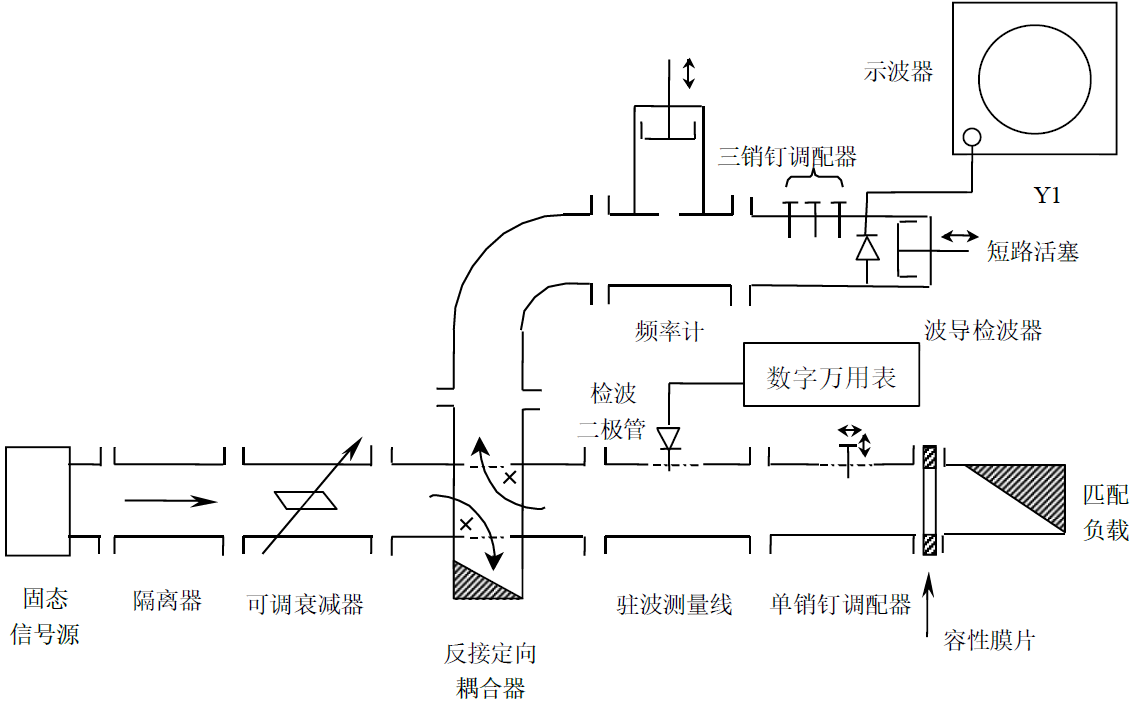
\includegraphics[width = 0.9\textwidth]{pic/1-4.png}
                \caption{}
            \end{figure}

        \subsection{阻抗匹配测量}
        在测量线与容性膜片+匹配负载之间串接一只单销钉调配器。见图。单销钉调配器是一个其销钉插入波导深度和纵向位置都可以调节的器件。
        \begin{enumerate}
            \item 调节衰减器衰减量,使示波器有足够的方波信号显示。
            \item 细心调节销钉调配器销钉的横向位置和插入波导的深度,使示波器上显示的信号最小(最好能到零)。进而提高示波器的灵敏度和增加输入功率,重复上一调节过程直到当示波器的灵敏度为最高和输入功率为最大且又在示波器上观察到的信号为最小为止,即找到最佳匹配位置。
            \item 适当增加可调衰减器的衰减量之后,横向移动驻波测量线,记录该输入功率下数字万用表上的 max(匹配) P 与 min(匹配) P ,并计算此时的驻波系数 。
        \end{enumerate}
        实验数据:$$P_{max(\mbox{匹配})} = \qquad P_{min(\mbox{匹配})} = \qquad$$


    \section{实验结果分析}
        \subsection{计算波导波长$\lambda$}
        \subsection{计算$TE_{10}$模的波导波长$\lambda_E$,并比较}
        \subsection{计算$\rho $,读出$\Gamma $和归一化阻抗值。}
        \subsection{计算用单销钉调节匹配后的驻波系数。}
        \subsection{,计算匹配状态时销钉所呈现的归一化电抗值。}

        \subsection{回答问题:}
            \subsubsection{}
            \subsubsection{}
            \subsubsection{}
            \subsubsection{}
            \subsubsection{}

    \section{实验总结与心得体会}
    $h[n]=\frac{\sin \left[w_{0}\left(n-n_{0}\right)\right]}{\pi\left(n-n_{0}\right)}$
\end{document}